\documentclass{article}

\usepackage{graphicx}
\usepackage{tikz}
\usepackage{tikzsymbols}
\usetikzlibrary{calc,patterns,shapes.geometric}
\pagestyle{empty}
\usepackage[margin=0pt]{geometry}
\geometry{papersize={14in,12in}}

\def\centerarc[#1](#2)(#3:#4:#5){\draw[#1] ($(#2)+({#5*cos(#3)},{#5*sin(#3)})$) arc (#3:#4:#5);}

\begin{document}
	\begin{figure}
		\centering
		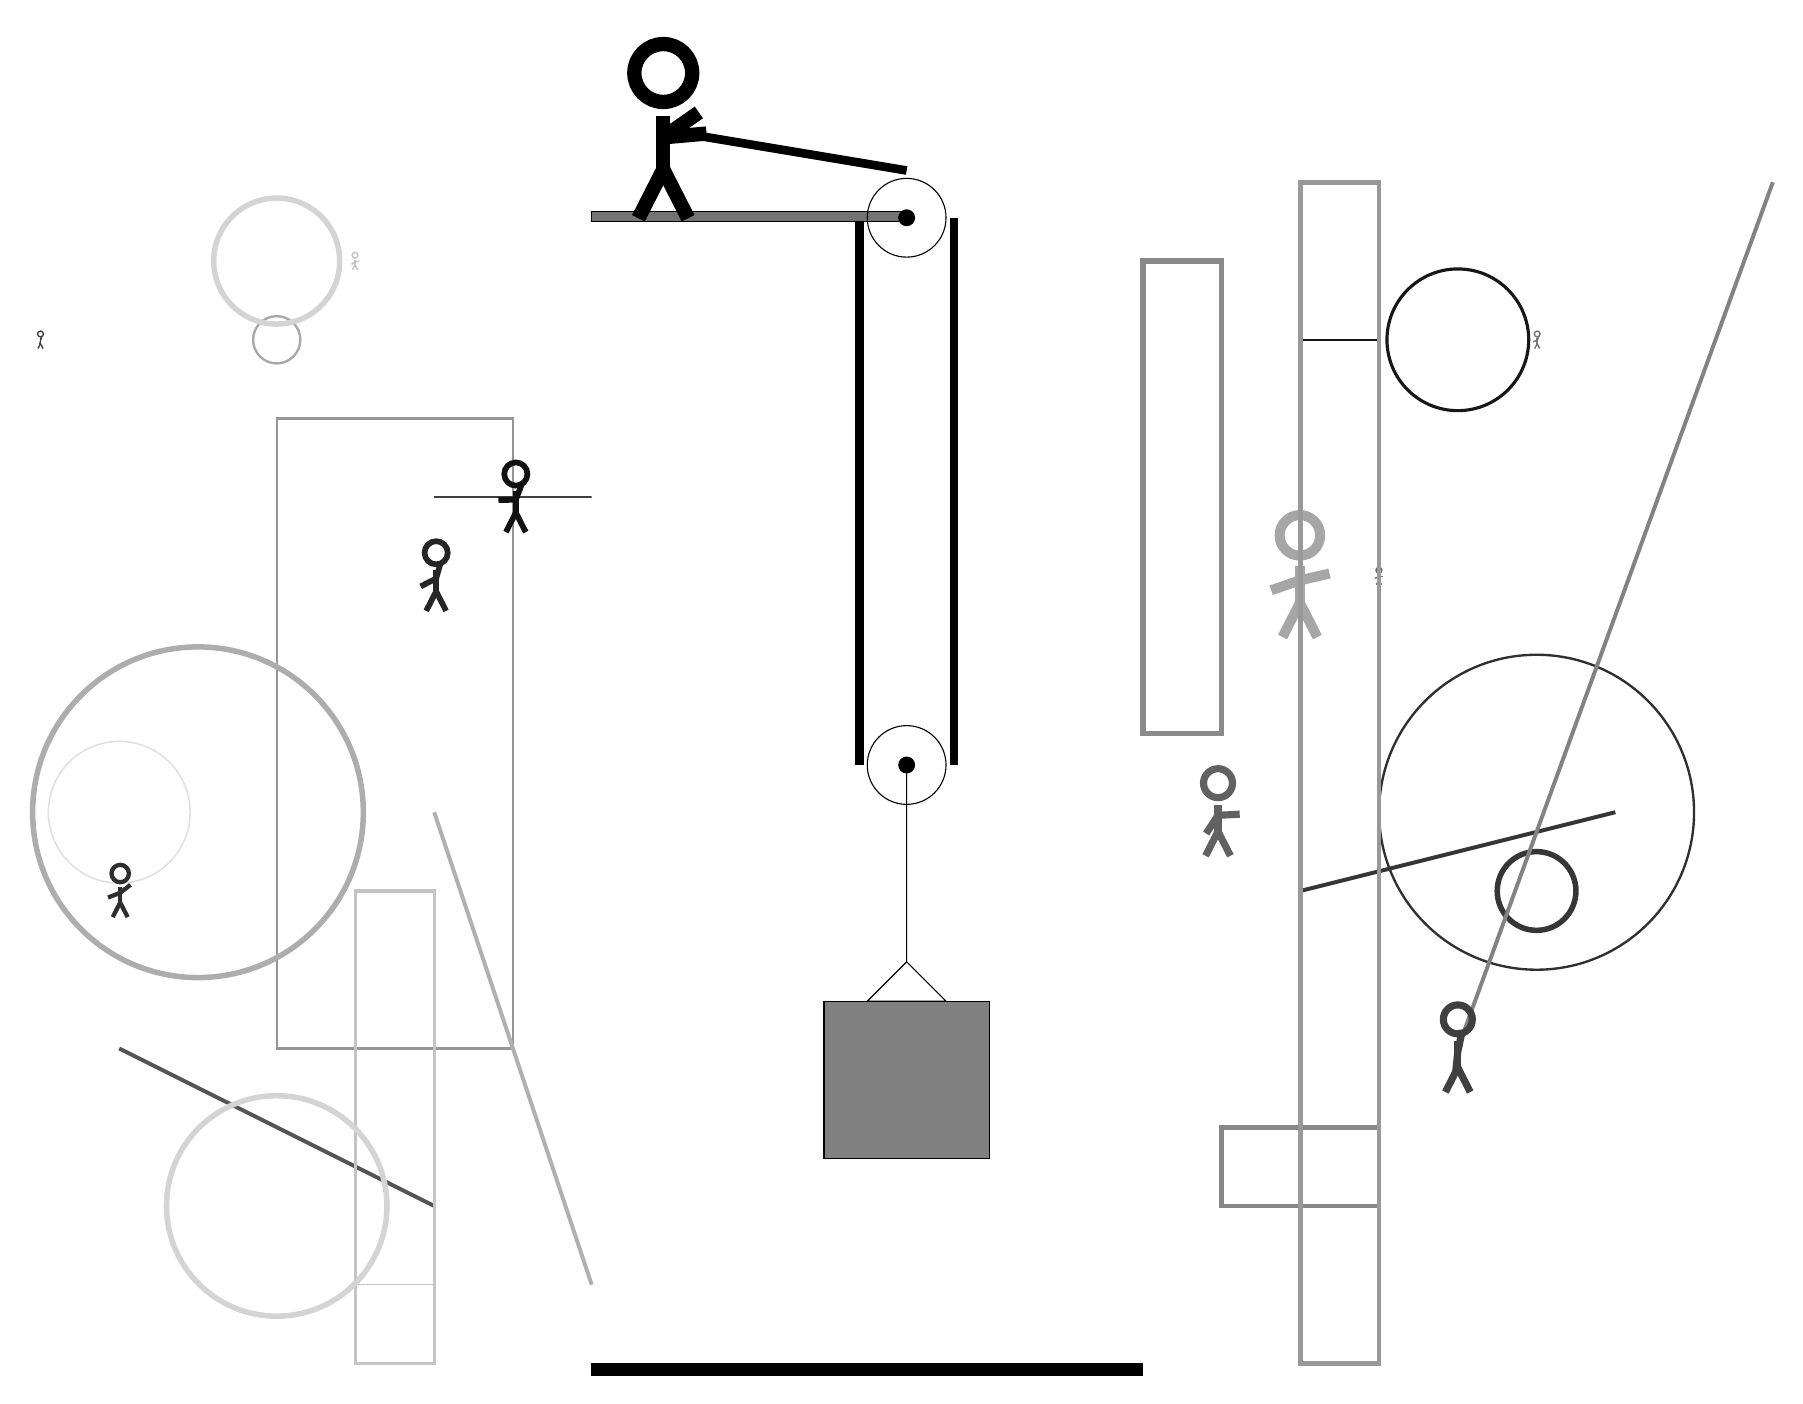
\begin{tikzpicture}
			%%%%% START %%%%%
			
			\draw[fill=black!55] (-2, 11.5) rectangle (2, 11.625);
			
			\draw (2, 4.6) circle (0.5);
			\draw[fill=black] (2, 4.6) circle (0.1);
			
			\draw (2, 11.55) circle (0.5);
			\draw[fill=black] (2, 11.55) circle (0.1);
			
			\draw (2, 4.6) -- (2, 2.1) -- (1.5, 1.6) -- (2.5, 1.6) -- (2, 2.1);
			\draw[fill=black!50] (0.95, 1.6) rectangle (3.05, -0.4);
			
			\draw[line width=1.1mm] (1.4, 11.5) -- (1.4, 4.6);
			\centerarc[line width=1.1mm](2, 4.6)(180:360:0.6);
			\draw[line width=1.1mm](2.6, 4.6) -- (2.6, 11.55);
			\centerarc[line width=1.1mm](2, 11.55)(0:90:0.6);
			\draw[line width=1.1mm](2, 12.15) -- (-1, 12.65);
			
			\node at (-1, 12.65) {\Strichmaxerl[10][-175][35]};
			
			\draw [line width=0.4mm, color=black!91](9, 10) circle (0.9);
			
			\node[line width=0.2mm, color=black!35] at (7, 7) {\Strichmaxerl[7][19][13]};
			\draw[line width=0.2mm, color=black!23] (-4, -2) rectangle (-5, -3);
			\draw [line width=0.3mm, color=black!81](10, 4) circle (2.0);
			\draw [line width=0.3mm, color=black!34](-6, 10) circle (0.3);
			
			\draw[line width=0.2mm, color=black!92] (7, 10) rectangle (8, -3);
			
			\node[line width=0.5mm, color=black!85] at (-4, 7) {\Strichmaxerl[4][27][74]};
			
			\node[line width=0.4mm, color=black!62] at (6, 4) {\Strichmaxerl[5][57][3]};
			\draw [line width=0.7mm, color=black!79](10, 3) circle (0.5);
			\draw[line width=0.5mm, color=black!79](7, 3) -- (11, 4);
			
			\node[line width=0.7mm, color=black!55] at (10, 10) {\Strichmaxerl[1][17][69]};
			
			\draw[line width=0.6mm, color=black!35] (-4, 2) rectangle (-4, 2);
			\draw[line width=0.6mm, color=black!47] (6, 0) rectangle (8, -1);
			\draw[line width=0.7mm, color=black!46] (5, 11) rectangle (6, 5);
			\draw[line width=0.3mm, color=black!41] (-3, 1) rectangle (-6, 9);
			\draw [line width=0.2mm, color=black!12](-8, 4) circle (0.9);
			
			\draw [line width=0.7mm, color=black!17](-6, 11) circle (0.8);
			\draw [line width=0.7mm, color=black!32](-7, 4) circle (2.1);
			\draw[line width=0.5mm, color=black!67](-4, -1) -- (-8, 1);
			\draw[line width=0.5mm, color=black!31](-4, 4) -- (-2, -2);
			\draw[line width=0.3mm, color=black!75] (-4, 8) rectangle (-2, 8);
			\node[line width=0.4mm, color=black!74] at (-9, 10) {\Strichmaxerl[1][80][71]};
			\node[line width=0.3mm, color=black!59] at (8, 7) {\Strichmaxerl[1][24][0]};
			\draw[line width=0.5mm, color=black!49](9, 1) -- (13, 12);
			\draw[line width=0.4mm, color=black!23] (-4, -3) rectangle (-5, 3);
			
			\draw [line width=0.7mm, color=black!17](-6, -1) circle (1.4);
			\node[line width=0.2mm, color=black!24] at (-5, 11) {\Strichmaxerl[1][38][4]};
			\draw[line width=0.7mm, color=black!65] (-2, 9) rectangle (-2, 9);
			\node[line width=0.7mm, color=black!75] at (9, 1) {\Strichmaxerl[5][84][78]};
			\node[line width=0.7mm, color=black!93] at (-3, 8) {\Strichmaxerl[4][1][69]};
			\draw[line width=0.6mm, color=black!40] (7, -3) rectangle (8, 12);
			
			\node[line width=0.5mm, color=black!82] at (-8, 3) {\Strichmaxerl[3][21][38]};
			
			\draw[fill=black] (-2, -3) rectangle (5, -3.15);
			
			%%%%% END %%%%%
		\end{tikzpicture}
	\end{figure}	
\end{document}